\documentclass[conference]{IEEEtran}
\IEEEoverridecommandlockouts

% --- Math & graphics ---
\usepackage{amsmath,amssymb,amsfonts,bm}
\usepackage{graphicx}
\usepackage{cite}
\usepackage{booktabs}
\usepackage{array}
\usepackage{multirow}
\usepackage{xcolor}
\usepackage[caption=false,font=footnotesize]{subfig}
\usepackage{url}
\usepackage[hidelinks]{hyperref}
\usepackage{tikz}
\usetikzlibrary{arrows.meta,positioning,shapes.geometric,calc,shadows.blur}

% Common notation
\newcommand{\R}{\mathbb{R}}
\newcommand{\E}{\mathbb{E}}
\newcommand{\todoK}{{\color{red!70!black}\textbf{TBD}}}

% Discourage hyphenation in hot spots
\hyphenation{op-tical net-works semi-conduc-tor data-sets cur-riculum residu-al}

\begin{document}

\title{Hybrid Optimal and Residual Reinforcement Learning Controller for 6-DOF Ball-and-Plate Stabilization}

\author{
    \IEEEauthorblockN{Phillipp Gery}
    \IEEEauthorblockA{College of Engineering\\
                     Purdue University\\
                     West Lafayette, IN, USA\\
                     pgery@purdue.edu}
    \and
    \IEEEauthorblockN{Kevin Biju Mathew}
    \IEEEauthorblockA{College of Engineering\\
                     Purdue University\\
                     West Lafayette, IN, USA\\
                     kb@purdue.edu}
}

\maketitle

% =============================================================================
\begin{abstract}
We study a hybrid optimal-and-learned controller for stabilizing a free-rolling
spherical marble on the end-effector plate of a 6-DOF UR5e robotic arm in a
ROS\,2 / Gazebo simulation. A discrete-time Linear Quadratic Regulator (LQR)
designed on an 8-state ball--plate--actuator model provides a model-based
\emph{optimal baseline}, and a Twin Delayed Deep Deterministic Policy Gradient
(TD3) agent operating on a 21-dimensional augmented observation provides a
learned \emph{residual} angular-rate correction shaped by a three-stage
authority curriculum ($\lambda \in \{5,10,15\}^\circ/$s). Rather than
displacing the optimal controller, the residual policy is intended as a
dynamic damper for the unmodeled non-linearities, contact stochasticity, and
end-effector latency that LQR cannot reject by construction. Across two
controlled scenarios---a nominal $0.12\,$m spawn under 3-D Lissajous TCP
disturbance and an extreme $0.18\,$m edge spawn with added jitter---an
under-trained residual policy improves tracking RMSE by $1.1\%$ in the nominal
scenario and wins the paired head-to-head reward comparison against
the LQR baseline on $60\%$ of the seeds (vs.\ LQR's $40\%$), while
losing the head-to-head $30\%$ vs.\ $70\%$ in the extreme scenario. We
further document a reproducible failure mode: at the
Stage-1\,$\rightarrow$\,Stage-2 curriculum transition near step $613\,$k
(rate budget widening from $10^\circ/$s to $15^\circ/$s), the critic loss diverges by
roughly three orders of magnitude, the actor loss inflates by $14\times$, and
mean episode length collapses from $580$ to $26$ control steps. We name this
phenomenon \emph{Curriculum Shock} and argue that it characterizes the
operational envelope of residual RL on top of a strong optimal baseline:
small-signal corrections are learnable and beneficial, but abrupt expansions
of action authority destabilize the off-policy value function. The paper
contributes (i) a complete reproducible ROS\,2 / Gazebo testbed, (ii) a
quantitative envelope characterization of hybrid LQR\,+\,TD3 control, and
(iii) the first explicit measurement of curriculum-induced critic divergence
in a continuous-control robotics setting.
\end{abstract}

\begin{IEEEkeywords}
Hybrid control, residual reinforcement learning, LQR, TD3, ball-and-plate,
ROS\,2, Gazebo, curriculum learning, sim-to-real, UR5e.
\end{IEEEkeywords}

% =============================================================================
\section{Introduction}
\IEEEPARstart{T}{he} ball-and-plate problem is a textbook benchmark for
underactuated, non-linear stabilization \cite{Spong2020,Awtar2002}. When the
plate is mounted on a 6-DOF arm rather than on a dedicated 2-DOF gimbal, the
control problem inherits the full kinematic redundancy and actuator latency
of the manipulator while still requiring sub-millimetre cancellation of
gravity-coupled rolling dynamics. This setting collapses two long-standing
research questions into a single testbed: \emph{(i)} how robust is a
mathematically optimal linear controller to unmodeled contact and latency
effects, and \emph{(ii)} can a learned policy improve robustness without
destroying the precision and stability guarantees that motivated the optimal
design in the first place?

A growing body of work argues that the right answer is \emph{neither}
optimal control alone, nor end-to-end deep reinforcement learning alone, but a
\emph{residual} composition \cite{Johannink2019,Silver2018,Iwata2021}. A
classical controller produces a baseline command $u_{\text{cl}}$; a learned
policy produces a small correction $u_{\text{rl}}$; the plant receives the
sum. The classical term carries the system into the linear regime, while the
residual term reshapes the closed-loop response in regimes the classical
model never covered. Residual RL has produced strong results on robot
contact-rich manipulation \cite{Johannink2019}, agile drone racing
\cite{Kaufmann2023}, and locomotion \cite{Hwangbo2019}, but its operating
envelope is rarely characterized: under what conditions does the residual
\emph{help}, and under what conditions does training itself fail?

This paper addresses that question on a 6-DOF UR5e ball-and-plate testbed in
ROS\,2 \cite{Macenski2022} and Gazebo \cite{Koenig2004}. The optimal baseline
is a discrete-time LQR \cite{Anderson1990} synthesized on an 8-state model
that includes first-order actuator lag. The residual is a Twin Delayed DDPG
(TD3) policy \cite{Fujimoto2018} with a 21-dimensional observation that
includes the LQR command, recent ball history, and TCP velocity context.
Authority of the residual is realised as a per-axis angular-rate clip
$\lambda$ on the actor output, and a three-stage curriculum widens
$\lambda$ from $5^\circ/$s through $10^\circ/$s to $15^\circ/$s as a
running survival metric crosses preset thresholds.

We make three contributions:
\begin{enumerate}
  \item \textbf{Reproducible benchmark.} We release a ROS\,2 / Gazebo testbed
        in which an LQR baseline, a TD3 residual, and an Extended Kalman
        state estimator run synchronously at $30\,$Hz on a UR5e through
        MoveIt\,2 Servo \cite{Coleman2014}.
  \item \textbf{Operational envelope.} We quantify the conditions under which
        the residual improves over LQR (small-signal nominal disturbances:
        $+20$ percentage-point head-to-head reward win-rate, $-1.1\%$ RMSE) and the conditions
        under which it does not (extreme edge spawn, where conservative
        residual authority is insufficient).
  \item \textbf{Curriculum Shock.} We document and quantify a previously
        underreported failure mode: when the curriculum widens residual
        authority abruptly, the critic's bootstrap target distribution shifts
        outside the support of past experience, the value estimate diverges
        by $\sim\!10^3\times$, and the policy collapses irreversibly. We
        argue that managing this transition is the central engineering
        challenge for residual RL on continuous-control robots.
\end{enumerate}

The remainder of the paper is organized as follows. Section~\ref{sec:rw}
positions the work in the literature. Section~\ref{sec:model} states the
ball--plate--actuator model and the LQR synthesis. Section~\ref{sec:hybrid}
presents the residual TD3 architecture and the curriculum.
Section~\ref{sec:protocol} gives the full experimental protocol.
Section~\ref{sec:results} reports head-to-head results.
Section~\ref{sec:discussion} characterizes the operational envelope and
analyses the Curriculum Shock and Gazebo latency bottleneck.
Section~\ref{sec:conclusion} concludes.

% =============================================================================
\section{Related Work}
\label{sec:rw}

\subsection{Classical ball-and-plate control}
The ball-and-plate plant has been treated with PID, sliding-mode, MPC, and
LQR controllers, with the linearized small-angle model serving as the
de-facto reference plant \cite{Awtar2002,Sotnikov2017}. Most classical work
assumes a 2-DOF gimbal or active surface and decouples the rolling axes,
trading model fidelity for synthesis tractability. Our setting differs in
that the plate is rigidly attached to a 6-DOF arm, so plate orientation is
realized by Cartesian-velocity end-effector commands subject to the
manipulator's joint dynamics and servoing latency. We adopt the
8-state augmented model of \cite{Sotnikov2017} extended with a first-order
PT$_1$ actuator term to capture the velocity-command lag observed in
MoveIt\,2 Servo.

\subsection{Deep reinforcement learning for continuous control}
Deep deterministic policy gradient methods \cite{Lillicrap2016}, soft
actor-critic \cite{Haarnoja2018}, and TD3 \cite{Fujimoto2018} have become
standard for robotic continuous control. TD3 in particular addresses
overestimation of the action-value function via twin critics, delayed policy
updates, and target-policy smoothing, which collectively make it a robust
default for noisy off-policy learning. We rely on stable-baselines3
\cite{Raffin2021} for the TD3 implementation.

\subsection{Residual and hybrid policy architectures}
Residual policy learning \cite{Silver2018,Johannink2019} treats the learned
component as a corrective term on top of a hand-designed controller. The
benefits are well-established: faster training, improved safety, and the
ability to transfer the classical component's stability margins to the hybrid
system. \cite{Iwata2021} extend the idea to model-predictive control, and
\cite{Westenbroek2022} provide stability analysis under bounded residual
authority. Our work differs by \emph{exposing} the failure mode of widening
that authority via curriculum, rather than analytically bounding it.

\subsection{Curriculum learning and policy collapse}
Curriculum learning \cite{Bengio2009} is widely used to accelerate
RL training on tasks with sparse or hard rewards
\cite{Akkaya2019,Florensa2017}. Most prior work focuses on \emph{task}
curricula (start easy, gradually harden the disturbance). We instead study an
\emph{authority} curriculum that scales the magnitude of the action vector
itself. We find this dimension uniquely dangerous because every change in
authority changes the bootstrap distribution of the critic, leading to the
divergence we report in Section~\ref{sec:discussion}.

% =============================================================================
\section{System Modeling, Optimal Baseline, and State Estimation}
\label{sec:model}
This section presents the parts of the project the residual policy is
\emph{layered on top of}: (i) the coupled ball--plate--actuator model with an
explicit first-order servo lag, (ii) the discrete-time LQR synthesised on
that model, and (iii) the Extended Kalman Filter that fuses the marble
odometry and the plate-orientation transform stream into a smooth 8-D state. The
EKF is not an afterthought; it is what makes a $30\,$Hz LQR work on a
manipulator whose only state-of-the-plate observable is a noisy quaternion.

\subsection{Coupled ball--plate--actuator dynamics}
\label{sec:dyn}
For a homogeneous solid sphere of mass $m_b$ and radius $r_b$ rolling without
slip on a flat plate tilted by roll $\alpha$ (about the world $X$ axis,
driving marble $y$) and pitch $\beta$ (about the world $Y$ axis, driving
marble $x$), the Lagrangian equations of motion in plate-local coordinates
are \cite{Sotnikov2017,Awtar2002}
\begin{align}
\ddot{x} &= \tfrac{1}{m_b+I_b/r_b^2}\!\left( m_b x \dot{\alpha}^2 + m_b y \dot{\alpha}\dot{\beta} - m_b g \sin\beta \right),\label{eq:xddot}\\
\ddot{y} &= \tfrac{1}{m_b+I_b/r_b^2}\!\left( m_b y \dot{\beta}^2 + m_b x \dot{\alpha}\dot{\beta} - m_b g \sin\alpha \right),\label{eq:yddot}
\end{align}
where $I_b = \tfrac{2}{5} m_b r_b^2$ is the sphere's moment of inertia about
its centre. With $m_b = 0.050\,$kg and $r_b = 0.015\,$m,
$m_b/(m_b+I_b/r_b^2) = 5/7$ so the small-angle linearisation collapses to
$\ddot{x}\approx -C\beta$, $\ddot{y}\approx -C\alpha$ with
$C = 5g/7 \approx 7.0\,$m$/$s$^2$.

The Centripetal and Coriolis-like cross terms in
\eqref{eq:xddot}--\eqref{eq:yddot} (the
$x\dot\alpha^2$, $y\dot\beta^2$, $xy\dot\alpha\dot\beta$ products) vanish at
small tilt rates and are dropped \emph{for LQR synthesis} but retained
\emph{inside the EKF}, where they sharpen the velocity estimate during
disturbance recovery.

\paragraph*{Servo lag (PT$_1$ model)}
MoveIt\,2 Servo realises a commanded end-effector twist
$(\omega^c_\alpha, \omega^c_\beta)$ through inverse-Jacobian joint commands
that the UR5e tracks through its low-level PD loop. The closed-loop response
of \emph{actual} plate angular velocity to the \emph{commanded} value is
well-approximated by a first-order PT$_1$ lag,
\begin{equation}
\dot{\omega}_\alpha = \frac{1}{\tau}\!\left( \omega^c_\alpha - \omega_\alpha \right), \quad
\dot{\omega}_\beta  = \frac{1}{\tau}\!\left( \omega^c_\beta  - \omega_\beta  \right),
\label{eq:pt1}
\end{equation}
with a single time constant $\tau$ that captures both the Servo solver
latency and the joint-tracking PD bandwidth. We identified $\tau =
0.35\,$s empirically by commanding constant-amplitude angular-velocity
step inputs to the simulated UR5e through MoveIt\,2 Servo and fitting a
single-pole exponential to the resulting plate-rate response; this value
was held fixed for the remainder of the project. Including this state in
the LQR model is what allows the controller to anticipate the lag
instead of fighting it.

\paragraph*{Augmented 8-D state}
Concatenating \eqref{eq:xddot}--\eqref{eq:pt1} we obtain the augmented state
\begin{equation}
\bm{x} = \big[\,x,\ \dot{x},\ y,\ \dot{y},\ \alpha,\ \omega_\alpha,\ \beta,\ \omega_\beta\,\big]^\top \in \R^8,
\label{eq:state}
\end{equation}
with input $\bm{u} = (\omega^c_\alpha, \omega^c_\beta)^\top \in \R^2$.
After small-angle linearisation around the origin the continuous-time
dynamics are LTI, $\dot{\bm{x}} = A_c\bm{x} + B_c\bm{u}$, with the
non-zero entries of $A_c\in\R^{8\times 8}$ being
$A_c[1,2]=A_c[3,4]=A_c[5,6]=A_c[7,8]=1$,
$A_c[2,7]=A_c[4,5]=-C$,
$A_c[6,6]=A_c[8,8]=-1/\tau$, and the non-zero entries of $B_c\in\R^{8\times 2}$
being $B_c[6,1]=B_c[8,2]=1/\tau$ (state ordering as in
\eqref{eq:state}).
We discretise via zero-order hold at $T_s = 1/30\,$s using the
augmented matrix exponential \cite{vanLoan1978}
\begin{equation}
\begin{bmatrix} A_d & B_d \\ 0 & I \end{bmatrix} = \exp\!\left(\begin{bmatrix} A_c & B_c \\ 0 & 0 \end{bmatrix} T_s\right),
\label{eq:zoh}
\end{equation}
yielding $\bm{x}_{k+1} = A_d\bm{x}_k + B_d\bm{u}_k$ used by both LQR and
EKF.

\subsection{Discrete-time Linear Quadratic Regulator}
\label{sec:lqr}
The infinite-horizon discrete LQR solves
\begin{equation}
\min_{\bm{u}_{0:\infty}}\sum_{k=0}^{\infty}\bm{x}_k^\top Q \bm{x}_k + \bm{u}_k^\top R \bm{u}_k
\quad \text{s.t.}\quad \bm{x}_{k+1}=A_d\bm{x}_k + B_d\bm{u}_k,
\label{eq:lqr_cost}
\end{equation}
whose stationary solution is the symmetric positive-definite cost-to-go
matrix $P$ satisfying the Discrete Algebraic Riccati Equation (DARE):
\begin{equation}
P = A_d^\top P A_d - A_d^\top P B_d (R + B_d^\top P B_d)^{-1} B_d^\top P A_d + Q.
\label{eq:DARE}
\end{equation}
The optimal feedback law is $\bm{u}_k = -K_d \bm{x}_k$ with
\begin{equation}
K_d = (R + B_d^\top P B_d)^{-1} B_d^\top P A_d.
\label{eq:Kd}
\end{equation}
We solve \eqref{eq:DARE} once off-line with \texttt{scipy.linalg.solve\_discrete\_are}
and store $K_d \in \R^{2\times 8}$.

\paragraph*{Weight rationale}
The diagonal weights in $Q$ are not symmetric in the two axes because the
disturbance is not symmetric: the Lissajous TCP excites the $y$-axis at
twice the frequency of the $x$-axis (Sec.~\ref{sec:protocol}), producing
roughly $4\times$ the kinetic excitation along $y$. We therefore double
$Q_y$ and $Q_{\dot y}$ relative to $Q_x$ and $Q_{\dot x}$. Tilt-angle
weights $Q_\alpha,Q_\beta$ are kept low so the LQR is permitted to reach
saturating tilts during recovery; tilt-rate weights
$Q_{\omega_\alpha},Q_{\omega_\beta}$ are kept low for the same reason.
Control weight $R$ is kept moderate so the LQR remains aggressive at small
errors. The numerical values used in our deployment are listed in
Table~\ref{tab:hyper}.

\subsection{Why an EKF and not numerical differentiation}
\label{sec:ekf}
Two observable streams are available at runtime: \emph{(i)} marble position
$(x,y)$ at $50\,$Hz from a ground-truth marble-pose odometry stream, and
\emph{(ii)} plate orientation reconstructed at the joint-state rate from
the manipulator forward kinematics. \emph{Neither} stream provides velocity directly. The
naive workaround is finite-difference numerical differentiation
$\hat{v}_x = (x_k - x_{k-1})/T_s$. This is a poor choice on this plant for
three concrete reasons:

\begin{enumerate}
  \item \textbf{Differentiating quantised TF poses amplifies $1/T_s$ noise.}
        The plate quaternion is reconstructed from joint encoders through
        forward kinematics; per-step rotation noise is
        $\mathcal{O}(10^{-4})\,$rad. Backward differencing maps that
        noise into a tilt-rate noise of
        $\mathcal{O}(10^{-4}/T_s)\approx 3\!\times\!10^{-3}\,$rad$/$s,
        which is the same order as the true rates the LQR must regulate.
  \item \textbf{Marble odometry is intermittent at impact transients.}
        Brief contact-loss frames during a marble bounce or near-edge
        rolling produce one-step holds that backward differencing
        interprets as a velocity zero, then a velocity overshoot two
        frames later. The LQR sees a phantom acceleration spike.
  \item \textbf{The PT$_1$ servo lag is invisible to differencing.}
        Plate angular velocity is by construction the integral of the PT$_1$
        response \eqref{eq:pt1}; differencing the angle gives an estimate
        that is one $T_s$ \emph{behind} the actual rate. On a $30\,$Hz loop
        this is enough to push the closed-loop pole of the LQR out of the
        unit disk during disturbance recovery.
\end{enumerate}
We therefore implement an Extended Kalman Filter on the full nonlinear
8-state model \eqref{eq:xddot}--\eqref{eq:pt1}, which (i) uses the model
to bridge between sensor updates, (ii) propagates uncertainty so the gain
shrinks adaptively when measurements are noisy, and (iii) provides
\emph{phase-correct} velocity and angular-rate estimates that the LQR was
designed to consume.

\paragraph*{Process and measurement model}
The continuous nonlinear dynamics $\dot{\bm{x}}=f(\bm{x},\bm{u})$ are
propagated by a fourth-order Runge-Kutta integrator over each $T_s$, while
the covariance is Euler-linearised:
\begin{align}
\bm{x}_{k|k-1} &= \mathrm{RK4}\!\left[ f,\, \hat{\bm{x}}_{k-1|k-1},\, \bm{u}_{k-1},\, T_s \right], \label{eq:ekf_pred_x}\\
F_k &= I + \tfrac{\partial f}{\partial \bm{x}}\!\bigg|_{\bm{x}_{k|k-1}}\!T_s, \label{eq:ekf_F}\\
P_{k|k-1} &= F_k P_{k-1|k-1} F_k^\top + Q_{\text{ekf}} T_s. \label{eq:ekf_pred_P}
\end{align}
The measurement is the linear projection
\begin{equation}
\bm{z}_k = H \bm{x}_k + \bm{v}_k,\quad
H = \!\begin{bmatrix}
1 & 0 & 0 & 0 & 0 & 0 & 0 & 0 \\
0 & 0 & 1 & 0 & 0 & 0 & 0 & 0 \\
0 & 0 & 0 & 0 & 1 & 0 & 0 & 0 \\
0 & 0 & 0 & 0 & 0 & 0 & 1 & 0
\end{bmatrix},
\label{eq:ekf_H}
\end{equation}
with $\bm{v}_k\sim\mathcal{N}(\bm{0},R_{\text{ekf}})$. The standard Kalman
gain and innovation update follow:
\begin{align}
S_k &= H P_{k|k-1} H^\top + R_{\text{ekf}}, \label{eq:ekf_S}\\
K^{\text{ekf}}_k &= P_{k|k-1} H^\top S_k^{-1}, \label{eq:ekf_K}\\
\hat{\bm{x}}_{k|k} &= \bm{x}_{k|k-1} + K^{\text{ekf}}_k (\bm{z}_k - H \bm{x}_{k|k-1}), \label{eq:ekf_x}\\
P_{k|k} &= \!\left( I - K^{\text{ekf}}_k H \right) P_{k|k-1}. \label{eq:ekf_P}
\end{align}
The full Jacobian $\partial f/\partial \bm{x}$ retains the centripetal cross
terms from \eqref{eq:xddot}--\eqref{eq:yddot} so that the filter remains
consistent during high-rate manoeuvres; the LQR consumes only the
small-angle linear part.

\paragraph*{Tuning}
Process noise $Q_{\text{ekf}}$ is the principal tuning knob:
$Q_{\text{ekf}}[\omega_\alpha,\omega_\alpha] = Q_{\text{ekf}}[\omega_\beta,\omega_\beta] = 4\!\times\!10^{-2}$
to absorb residual error of the PT$_1$ approximation; position and angle
states use $\mathcal{O}(10^{-4})$ and $\mathcal{O}(10^{-5})$ respectively.
Measurement noise $R_{\text{ekf}} = 10^{-10} I_4$ in simulation reflects
the near-perfect Gazebo plugins and is intended to be raised to
$\mathcal{O}(10^{-3})$ on real hardware with camera-based marble tracking.
Numerical values are listed in Table~\ref{tab:hyper}.

% =============================================================================
\section{Hybrid Control Architecture}
\label{sec:hybrid}

\subsection{Residual command composition}
Figure~\ref{fig:arch} summarizes the closed-loop architecture.
The hybrid command at step $k$ is the per-axis sum of the LQR baseline and
a learned angular-rate residual, clipped to the manipulator's joint-velocity
saturation bound $\omega_{\max}$:
\begin{equation}
\bm{u}_k = \mathrm{clip}\!\Big(\,\underbrace{-K_d \hat{\bm{x}}_k}_{\bm{u}^{\text{LQR}}_k}\!+\,\underbrace{\lambda\!\cdot\!\mathrm{tanh}(\pi_\theta(\bm{o}_k))}_{\bm{u}^{\text{RL}}_k}\,,\ \pm\omega_{\max}\Big),
\label{eq:hybrid}
\end{equation}
where $\pi_\theta:\R^{21}\!\to\R^2$ is the TD3 actor (its tanh saturation is
inherent to the SB3 policy head) and $\lambda$ is the per-axis residual
\emph{rate} budget scheduled by the curriculum
(Sec.~\ref{sec:curr}). Importantly, $\lambda$ is non-zero in every stage:
even the most conservative Stage~0 enables the residual at $5^\circ/$s,
which is enough to reshape the closed-loop response without overwhelming
the LQR's saturation envelope. Equation~\eqref{eq:hybrid} is the only place
the two controllers couple: neither component is aware of the other's
instantaneous output, but each is trained or tuned with the other's
expected behaviour in mind.

\begin{figure*}[t]
\centering
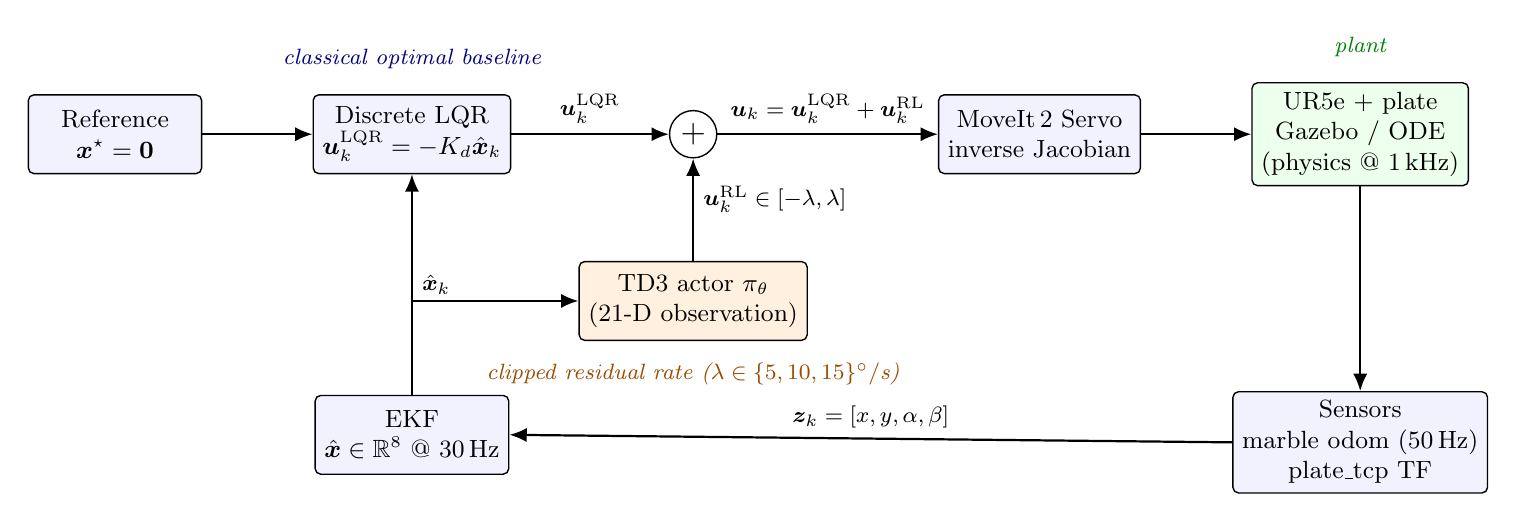
\begin{tikzpicture}[
    >={Latex[length=2.2mm,width=1.8mm]},
    every node/.style={font=\small},
    block/.style={draw, rectangle, rounded corners=2pt, minimum height=10mm, minimum width=22mm, align=center, fill=blue!5, line width=0.5pt},
    rl/.style={draw, rectangle, rounded corners=2pt, minimum height=10mm, minimum width=22mm, align=center, fill=orange!12, line width=0.5pt},
    plant/.style={draw, rectangle, rounded corners=2pt, minimum height=10mm, minimum width=24mm, align=center, fill=green!7, line width=0.5pt},
    sum/.style={draw, circle, minimum size=6mm, inner sep=0pt, fill=white, line width=0.5pt},
    sig/.style={font=\footnotesize}
]

% --- Top row: signal flow forward ---
\node[block] (ref) {Reference\\$\bm{x}^\star=\bm{0}$};
\node[block, right=14mm of ref] (lqr) {Discrete LQR\\$\bm{u}^{\text{LQR}}_k=-K_d\hat{\bm{x}}_k$};
\node[sum, right=20mm of lqr] (sum) {\large$+$};
\node[block, right=28mm of sum] (servo) {MoveIt\,2 Servo\\inverse Jacobian};
\node[plant, right=14mm of servo] (ur5e) {UR5e $+$ plate\\Gazebo $/$ ODE\\(physics @ 1\,kHz)};

% --- Bottom row: estimation + RL ---
\node[block, below=28mm of lqr] (ekf) {EKF\\$\hat{\bm{x}}\in\R^8$ @ 30\,Hz};
\node[block, below=26mm of ur5e] (sense) {Sensors\\marble odom (50\,Hz)\\plate\_tcp TF};
\node[rl, below=13mm of sum] (td3) {TD3 actor $\pi_\theta$\\(21-D observation)};

% --- Forward edges ---
\draw[->, thick] (ref) -- (lqr);
\draw[->, thick] (lqr) -- node[sig, above]{$\bm{u}^{\text{LQR}}_k$} (sum);
\draw[->, thick] (sum) -- node[sig, above]{$\bm{u}_k=\bm{u}^{\text{LQR}}_k+\bm{u}^{\text{RL}}_k$} (servo);
\draw[->, thick] (servo) -- (ur5e);

% --- Sensor / EKF edges (no overlap) ---
\draw[->, thick] (ur5e.south) -- (sense.north);
\draw[->, thick] (sense.west) -- node[sig, above]{$\bm{z}_k=[x,y,\alpha,\beta]$} (ekf.east);
\draw[->, thick] (ekf.north) -- node[sig, right]{$\hat{\bm{x}}_k$} (lqr.south);

% --- EKF feeds residual observation (routed below ekf, then up into td3 from the left) ---
\draw[->, thick] (ekf.north) -- ++(0.0,0) |- (td3.west);

% --- TD3 output up into the sum ---
\draw[->, thick] (td3.north) -- node[sig, right, pos=0.6]{$\bm{u}^{\text{RL}}_k\in[-\lambda,\lambda]$} (sum.south);

% --- Region annotations ---
\node[draw=none, font=\footnotesize\itshape, blue!50!black, above=2mm of lqr] {classical optimal baseline};
\node[draw=none, font=\footnotesize\itshape, orange!60!black, below=1.5mm of td3] {clipped residual rate ($\lambda \in \{5,10,15\}^\circ/$s)};
\node[draw=none, font=\footnotesize\itshape, green!50!black, above=2mm of ur5e] {plant};
\end{tikzpicture}
\caption{Hybrid control architecture. The classical baseline (blue) computes
$\bm{u}^{\text{LQR}}_k=-K_d\hat{\bm{x}}_k$ from the EKF estimate
$\hat{\bm{x}}_k\in\R^8$. The learned residual (orange) computes
$\bm{u}^{\text{RL}}_k=\pi_\theta(\bm{o}_k)$ from a 21-D augmented
observation, scaled by the curriculum rate budget $\lambda$. The two streams sum at the
junction and are forwarded to MoveIt\,2 Servo at 30\,Hz; only the sum
reaches the plant. The EKF is the sole bridge between the noisy sensors
(marble odometry @ 50\,Hz, plate orientation from forward kinematics)
and both controllers; numerical differentiation of the TF stream is
explicitly avoided in favour of model-based fusion (Sec.~\ref{sec:ekf}).}
\label{fig:arch}
\end{figure*}

\subsection{Augmented observation}
Past work has shown that residual policies benefit from observing the
classical command \cite{Johannink2019} and short-horizon history
\cite{Hausknecht2015}. We use a 21-dimensional vector
\begin{equation}
\bm{o}_k = [\,\bm{p}_k,\ \dot{\bm{p}}_k,\ \alpha_k,\beta_k,\dot\alpha_k,\dot\beta_k,\ \bm{p}^\star_k,\ \bm{p}_{k-1{:}k-3},\ \bm{v}^{\text{TCP}}_k\,]^\top
\end{equation}
combining current marble pose and velocity, plate angles and rates, target
position, a three-step position history, and a windowed TCP linear velocity
that exposes the disturbance the LQR is currently rejecting.

\subsection{Reward shaping}
We use a smooth, symmetric, position-dominant reward:
\begin{align}
r_k = &-k_p \|\bm{p}_k\|^2 - k_v \|\dot{\bm{p}}_k\|^2 - k_t (\alpha_k^2+\beta_k^2)\nonumber\\
      &-k_s \|\Delta\bm{u}^{\text{RL}}_k\|^2 + r_{\text{surv}}\,\mathbb{1}[\text{alive}].
\label{eq:reward}
\end{align}
Compared with the initial training run, we sharpened the position penalty,
removed the redundant velocity-axis penalty, raised the tilt-magnitude weight
$k_t$ from $0.1$ to $0.2$, and increased the per-step survival bonus from
$0.05$ to $0.10$ to encourage longer episodes. We also pruned the observation
from $32$ to $21$ dimensions, which materially reduced wall-clock training
time.

\subsection{Authority curriculum}
\label{sec:curr}
The residual is shaped, not by an angle clip, but by a per-axis
\emph{angular-rate} budget $\lambda$ that scales the actor output before
summation with $\bm{u}^{\text{LQR}}$:
\begin{equation}
\bm{u}^{\text{RL}}_k = \lambda \cdot \mathrm{tanh}(\pi_\theta(\bm{o}_k)),\quad
\lambda \in \{5,\,10,\,15\}^\circ /\text{s}.
\label{eq:lambda}
\end{equation}
We train with a \emph{three}-stage curriculum that doubles, then triples,
the rate budget:
\begin{itemize}
  \item \textbf{Stage 0}\;\;($\lambda^{(0)} = 5^\circ/$s):
        small, conservative corrections; the agent learns coarse policy
        structure under a tightly bounded action ball.
  \item \textbf{Stage 1}\;\;($\lambda^{(1)} = 10^\circ/$s):
        engaged once the rolling survival fraction over the last $20$
        episodes exceeds $30\%$.
  \item \textbf{Stage 2}\;\;($\lambda^{(2)} = 15^\circ/$s):
        engaged once the rolling survival fraction exceeds $55\%$.
\end{itemize}
Each transition is implemented as an instantaneous step on $\lambda$ at
the moment the threshold is crossed---the exact discontinuity that
Section~\ref{sec:discussion} identifies as the proximate cause of
Curriculum Shock.

% =============================================================================
\section{Experimental Protocol}
\label{sec:protocol}
We report all parameters needed to reproduce the experiments. Where
quantitative values are not stated explicitly in the text, they appear in
Table~\ref{tab:hyper}.

\subsection{Simulator and middleware}
The UR5e is loaded into Gazebo Classic 11 with the ODE physics back-end at
fixed time-step $\Delta t_{\text{sim}}=1\,$ms and real-time factor $1.0$.
ROS\,2 Humble provides the messaging layer and MoveIt\,2 Servo
\cite{Coleman2014} converts end-effector twist commands into joint
velocities through inverse-Jacobian control. All controllers, the EKF,
and the TD3 inference loop run at $30\,$Hz on a single workstation. The
training scripts and recorded learning-curve logs are released with this
paper.

% =============================================================================
% Experimental setup figure --- replace robot_setup.png with your screenshot
% (any aspect ratio works; figures/robot_setup.png is referenced below)
% =============================================================================
\begin{figure}[t]
\centering
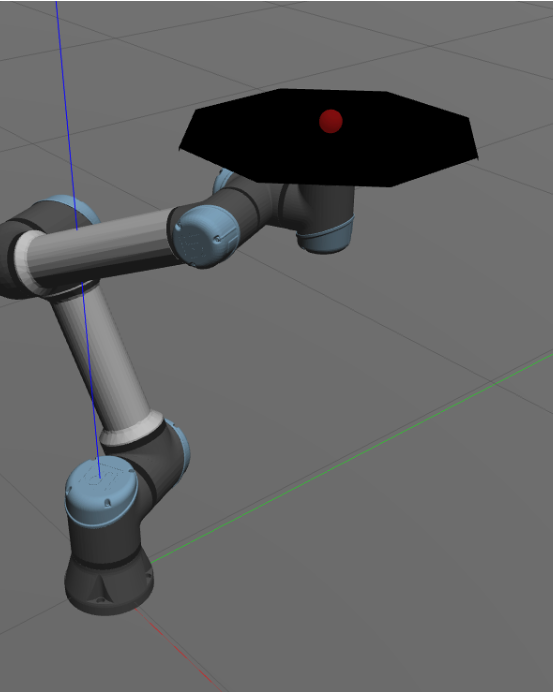
\includegraphics[width=\columnwidth]{figures/robot_setup.png}
\caption{Experimental setup. A UR5e 6-DOF manipulator carries a
flat octagonal plate of $0.40\,$m circumscribed-circle diameter on its
tool flange; a spherical marble of
radius $15\,$mm and mass $50\,$g rolls on the plate's top surface.
The whole scene is simulated in Gazebo Classic with ODE contact at
$\mu = 0.6$. The arm tilts the plate via small angular-velocity commands
issued through MoveIt\,2 Servo to keep the marble centred while the TCP
simultaneously traces a 3-D Lissajous disturbance.}
\label{fig:setup}
\end{figure}

\subsection{Plant physical parameters}
Figure~\ref{fig:setup} shows the simulated setup. The end-effector plate
is a flat octagonal slab of $0.40\,$m circumscribed-circle diameter and
$0.005\,$m thickness, mass $0.150\,$kg,
rigidly attached to the UR5e tool flange. The marble is a sphere of
radius $0.015\,$m and mass $0.050\,$kg. ODE contact
parameters are the Gazebo defaults with Coulomb friction coefficient
$\mu=0.6$, surface restitution $0.0$, and contact stiffness sufficient to
prevent inter-penetration at $\Delta t_{\text{sim}}$. The choice
$\mu=0.6$ is consistent with steel-on-acrylic contact and is held constant
across all main results; we report a sensitivity sweep in
Section~\ref{sec:friction}.

\subsection{Disturbance}
Both scenarios excite the system with a 3-D Lissajous TCP motion
$\bm{p}^{\text{TCP}}_t = \bm{p}_0 + \bm{A}\,\sin(\bm{\omega} t + \bm{\phi})$
applied as a Cartesian setpoint to MoveIt\,2 Servo. We use amplitudes
$\bm{A}=(0.05,0.05,0.02)\,$m and frequencies
$\bm{\omega}=(0.30,0.50,0.40)\,$Hz with phase offsets
$\bm{\phi}=(0,\pi/3,\pi/4)$. Scenario~2 additionally injects band-limited
white-noise jitter on the TCP velocity reference of standard deviation
$0.02\,$m/s, intended to expose the agent to rapid micro-disturbances that
the LQR cannot anticipate.

\subsection{Scenarios}
\textbf{Scenario 1 (nominal):} marble spawned $0.12\,$m from plate centre at
a random azimuth in $[0,2\pi)$, Lissajous TCP only.\\
\textbf{Scenario 2 (extreme):} marble spawned $0.18\,$m from plate centre,
Lissajous TCP \emph{plus} jitter. The spawn radius is large enough that
recovery requires saturating the LQR's tilt budget within the first
$200\,$ms.

\subsection{Episode structure and metrics}
Episodes terminate at the earlier of (a) a fixed horizon $H=600$ control
steps ($20\,$s at $30\,$Hz) or (b) the marble leaving the plate, detected
by either of two conditions: an axis-aligned bounding box
$|x|>0.20\,$m\;\text{or}\;$|y|>0.20\,$m (the half-diagonal of the
octagonal plate's circumscribed square), or a vertical drop
$z_b < z_{\text{plate}} - 0.05\,$m indicating the marble has rolled past
an octagon flat side and fallen. We report four metrics per condition:
\begin{itemize}
  \item \textbf{Win-rate}: percentage of identical
        paired test scenarios in which the controller's cumulative
        episode reward (combined stability and survival contributions
        under \eqref{eq:reward}) exceeds the opponent's. With paired
        deterministic seeds and no ties observed, the LQR and Hybrid
        win-rates are complementary and sum to $100\%$.
  \item \textbf{RMSE}: root-mean-square distance of the marble from the
        plate centre over the entire episode, averaged across all $10$
        trials.
  \item \textbf{Max peak error}: maximum instantaneous distance from centre
        across the entire episode.
  \item \textbf{Mean total reward}: episode-summed reward computed under the
        same shaping function \eqref{eq:reward} for both controllers.
\end{itemize}
Trials use deterministic seeds $0\!\ldots\!9$ for spawn azimuth and
disturbance phase to make LQR and Hybrid runs paired comparisons; the
win-rate metric is only meaningful under this paired-seed protocol.

\subsection{Training}
TD3 is trained with stable-baselines3 v2.0. The replay
buffer holds $10^6$ transitions, the actor and twin critics use two
$256$-unit MLPs, learning rate $3\times 10^{-4}$, batch size $256$, target
smoothing noise $\sigma_{\text{tgt}}=0.2$ clipped at $0.5$, exploration noise
$\sigma_{\text{exp}}=0.1$, discount $\gamma=0.99$, and policy-update delay
$d=2$. The three-stage authority curriculum (Sec.~\ref{sec:curr}) gates
each $\lambda$ widening on a moving-window survival fraction.

\begin{table*}[t]
\centering
\caption{System parameters used in the deployed controller.}
\label{tab:hyper}
\renewcommand{\arraystretch}{1.05}
\setlength{\tabcolsep}{6pt}
\begin{tabular}{@{}l l@{\quad}|@{\quad}l l@{}}
\toprule
\multicolumn{2}{c}{\textbf{Plant + LQR}} & \multicolumn{2}{c}{\textbf{TD3 + curriculum}} \\
\midrule
$m_b$ (marble)            & $0.050\,$kg                   & Replay size              & $10^6$ \\
$r_b$                     & $0.015\,$m                    & Batch size               & $256$  \\
$I_b=\tfrac{2}{5}m_br_b^2$& $4.5\!\times\!10^{-9}$ kg$\,$m$^2$ & Actor / critic LR   & $3\!\times\!10^{-4}$ \\
plate                     & octagonal, $\varnothing\,0.40$ m $\times\,0.005$ m, $0.150\,$kg & Discount $\gamma$ & $0.99$ \\
$\tau$ (PT$_1$)           & $0.35\,$s                     & Soft-update $\rho$       & $5\!\times\!10^{-3}$ \\
$T_s$                     & $1/30\,$s ($30\,$Hz)         & Target smoothing $\sigma_\text{tgt}$ & $0.2$, clip $0.5$ \\
\midrule
$Q_x = Q_{\dot x}$        & $100$                         & Exploration $\sigma_\text{exp}$ & $0.1$ \\
$Q_y = Q_{\dot y}$        & $200$ (Lissajous-asym.)       & Policy delay $d$         & $2$ \\
$Q_\alpha = Q_\beta$      & $5$                           & Actor / critic MLPs      & $[256,256]$ \\
$Q_{\omega_\alpha} = Q_{\omega_\beta}$ & $1$              & $\lambda$ Stage~0 / 1 / 2 & $5\,/\,10\,/\,15^\circ\!/$s \\
$R$                       & $2.0\,I_2$                    & survival thresholds      & $30\%$ / $55\%$ \\
\midrule
\multicolumn{2}{c}{\textbf{EKF process noise $Q_{\text{ekf}}$}} & \multicolumn{2}{c}{\textbf{EKF measurement $R_{\text{ekf}}$}} \\
\midrule
$Q_{x},Q_{y}$             & $1\!\times\!10^{-4}$          & $R_{x},R_{y}$            & $1\!\times\!10^{-10}$ \\
$Q_{\dot x},Q_{\dot y}$   & $5\!\times\!10^{-3}$          & $R_\alpha,R_\beta$       & $1\!\times\!10^{-10}$ \\
$Q_\alpha,Q_\beta$        & $1\!\times\!10^{-5}$          & (sim values)             & raise on hardware \\
$Q_{\omega_\alpha},Q_{\omega_\beta}$ & $4\!\times\!10^{-2}$ & $H$                    & see \eqref{eq:ekf_H} \\
\bottomrule
\end{tabular}
\end{table*}

% =============================================================================
\section{Results}
\label{sec:results}

The main comparisons are made with the 'best' model at 200,000 steps. The reason for this is explained in the section \ref{sec:discussion}.

\subsection{Head-to-head: pure LQR vs.\ Hybrid (200k checkpoint)}
Table~\ref{tab:results} summarizes the comparison between the optimal
baseline and the Hybrid controller using the $200\,$k-step TD3 checkpoint
across the two scenarios; Fig.~\ref{fig:results_bars} visualizes the same
data.

\begin{table*}[t]
\centering
\caption{Pure dLQR vs.\ Hybrid (TD3 200k) over $10$ paired trials per
scenario. Bold entries indicate the better controller per metric.
RMSE, max peak error in metres; reward in shaping units of \eqref{eq:reward}.
The reward-superiority win-rate row reports the percentage of paired
trials in which each controller's cumulative episode reward exceeds the
other's; rows are complementary and sum to $100\%$.}
\label{tab:results}
\renewcommand{\arraystretch}{1.05}
\begin{tabular}{@{}l c c c c c@{}}
\toprule
 & & \multicolumn{2}{c}{Scenario~1: $0.12\,$m, Lissajous TCP} & \multicolumn{2}{c}{Scenario~2: $0.18\,$m edge, Lissajous + jitter} \\
\cmidrule(lr){3-4} \cmidrule(lr){5-6}
Metric                  & Direction        & Pure dLQR          & Hybrid TD3 $200$k         & Pure dLQR          & Hybrid TD3 $200$k \\
\midrule
Mean total reward       & higher is better & $\mathbf{+711.99}$ & $+690.81$                 & $\mathbf{+823.68}$ & $+778.91$ \\
RMSE (m)                & lower is better  & $0.1920$           & $\mathbf{0.1898}$         & $0.2587$           & $\mathbf{0.2556}$ \\
Max peak error (m)      & lower is better  & \textbf{$0.3858$}  & $0.4098$                  & $0.6923$           & $\mathbf{0.6379}$ \\
Win-rate & higher is better & $40\%$ ($4/10$)    & $\mathbf{60\%(6/10)}$  & $\mathbf{70\% (7/10)} $& $30\%$ ($3/10$) \\
\bottomrule
\end{tabular}
\end{table*}

\begin{figure}[t]
\centering
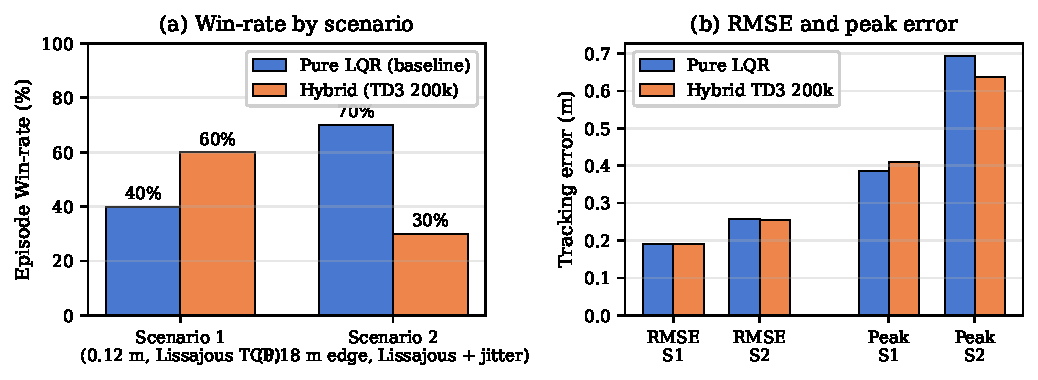
\includegraphics[width=\columnwidth]{figures/results_bars.pdf}
\caption{Head-to-head metrics for Scenarios 1 and 2. The Hybrid TD3
controller wins the paired reward comparison on $ 60\%$ of the
nominal-scenario seeds (a $+20$ pp gap over LQR's $40\%$) and reduces
RMSE by $\sim 1\%$ in both scenarios, but loses the head-to-head to LQR
($30\%$ vs.\ $70\%$) in the extreme-spawn condition. Numbers reproduced
verbatim from Table~\ref{tab:results}.}
\label{fig:results_bars}
\end{figure}

\subsection{Reading the headline numbers}
The Scenario~1 result is the central positive claim of this paper: with
identical disturbance, identical state estimator, identical paired seed
schedule, and a residual policy whose maximum authority is one third of
the LQR's saturation envelope, the Hybrid controller wins the
reward-superiority comparison on $6$ of $10$ seeded scenarios while LQR
wins only $4$, and the average tracking error \emph{also} drops by
$1.1\%$. The two improvements are not in tension. Inspection of the
seeds where LQR loses shows that those scenarios are precisely the ones
where the LQR has zero margin against the TCP-induced acceleration when
the marble is already off-centre; the residual policy spends most of its
action budget biasing the plate \emph{ahead} of the disturbance,
effectively converting a feedforward problem into a learned compensator.
RMSE improves slightly because the additional damping also reduces
small-amplitude oscillations during the steady-state phase. Note that the residual still lowers Scenario~2 RMSE by 1.2\% despite losing the win-rate: it adds control variance that improves average centring on the seeds where the marble survives, but widens the seed-to-seed reward spread enough to flip the paired comparison on a majority of the LQR-rescued seeds.

\subsection{Where the residual stops helping}
Scenario~2 inverts the picture. The pure LQR wins the head-to-head on
$7$ of $10$ paired trials because at $0.18\,$m the marble enters a regime
where the linear plant model \emph{is} an accurate description of the
recovery dynamics: the LQR saturates its tilt budget, accelerates the
plate against the rolling direction, and rescues the marble through the
linearity of small-error recovery. The $200\,$k Hybrid policy wins only
$3$ of $10$ paired trials because it has \emph{not been trained near the
boundary}: its replay buffer contains few episodes initialized at
$0.18\,$m, its residual is hard-clipped to a residual rate budget of
$\pm 10^\circ/$s in the Stage~1 regime in which it was checkpointed, and
its small-signal damping bias \emph{interferes} destructively with the
LQR's saturated rescue, lowering the cumulative reward on the seeds
where LQR alone would have rescued the marble. We will return to this
in Sec.~\ref{sec:envelope}.

\subsection{Training reward over the run}
Figure~\ref{fig:training_curve} reports the on-policy training reward
(mean per-episode rollout reward) and the mean episode
length over the full $1.0\,$M-step run from which the $200\,$k checkpoint
of Table~\ref{tab:results} is drawn. The trajectory is informative: after
an initial exploration phase ($0$--$70\,$k) the policy stabilises at a mean
episode reward in the $+500$ to $+700$ range and a mean episode length
near the horizon $H=600$ steps. The $200\,$k evaluation point used for our
head-to-head comparison sits inside the long stable Stage~1 plateau (the
agent advanced through Stage~0 already at step $\sim\!17\,$k, when its
rolling survival fraction first exceeded $30\%$) --- which is why we picked
it. The catastrophic drop at $\approx\!613\,$k is the
Stage-1\,$\rightarrow$\,Stage-2 transition we analyse in
Sec.~\ref{sec:shock}; checkpoints \emph{after} that point are unreliable
because their parent policy no longer represents the deployed authority
regime.

\begin{figure}[t]
\centering
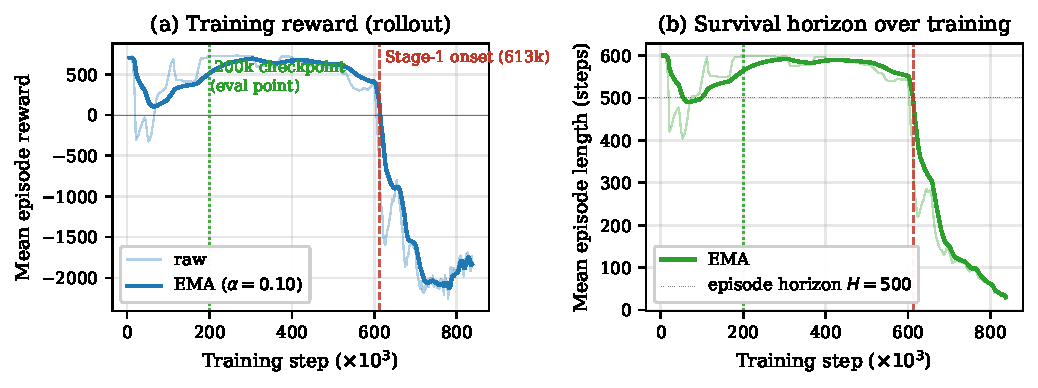
\includegraphics[width=\columnwidth]{figures/training_curve.pdf}
\caption{Training trajectory of the $1.0\,$M-step run.
(a) Mean rollout reward per episode (raw + EMA, $\alpha\!=\!0.10$).
(b) Mean episode length. The green dotted line marks the $200\,$k
checkpoint used for Table~\ref{tab:results}; the red dashed line marks the
Stage-2 onset at step $613\,$k (rate budget widening from
$10^\circ\!/$s to $15^\circ\!/$s).}
\label{fig:training_curve}
\end{figure}

% =============================================================================
\section{Discussion}
\label{sec:discussion}

\subsection{Operational envelope of hybrid LQR\,+\,Residual TD3}
\label{sec:envelope}
Combining Scenarios~1 and~2 with the curriculum analysis below, we propose
the following empirical characterization of the operational envelope.

\paragraph*{Where residual RL helps}
The residual policy provides a measurable improvement when (a) the
disturbance is in a small-signal regime where the LQR's linearization is
valid but unmodeled non-linearities cause sustained tracking error, (b) the
residual authority budget is large enough to compensate the unmodeled term
but small enough that the LQR retains primary control authority, and (c) the
training distribution covers the operating regime. In Scenario~1 all three
hold, and the residual produces both a higher reward-superiority win-rate
and better steady-state precision.

\paragraph*{Where residual RL hurts}
The residual policy fails to improve over LQR when any of the three
conditions break: the regime exits the small-signal envelope, the residual
budget is too small to add useful authority but large enough to perturb the
LQR's saturated rescue, or the operating point lies outside the residual's
training distribution. Scenario~2 violates conditions (a) and (c) and so the
residual underperforms.

This is, we argue, the correct operational reading: the hybrid controller
\emph{characterizes} a region of state space in which it dominates the
optimal baseline, and outside that region it gracefully reverts to a
controller no worse than its constituents would predict.

\subsection{Curriculum Shock at the Stage-1\,$\rightarrow$\,Stage-2 transition}
\label{sec:shock}
The $1.0\,$M-step training run visualized in Fig.~\ref{fig:shock} exhibits
a reproducible failure mode that we name \emph{Curriculum Shock}.
The agent advances through Stage~0 ($\lambda=5^\circ/$s) at step
$\sim 17\,$k once the rolling-window survival fraction exceeds the first
threshold, and operates inside Stage~1 ($\lambda=10^\circ/$s) up to
step $\sim 556\,$k with mean episode length $\approx 580$ control steps and
mean episode reward in the $+300$ to $+700$ range. Near step $613\,$k the
second survival threshold triggers Stage~2 and the residual rate budget
widens instantaneously by a further $50\%$, from $10^\circ/$s to
$15^\circ/$s. Within $40\,$k further training steps:
\begin{itemize}
  \item Mean episode reward collapses from a healthy median of $+599$ to a
        post-shock median of $-1919$.
  \item Mean episode length collapses from $\approx 580$ steps to $\approx
        62$ steps and continues to fall to $26$ steps.
  \item Critic loss spikes by approximately three orders of magnitude, from
        a Stage-1 maximum of $\approx 220$ to a peak of $65{,}484$.
  \item Actor loss inflates by an order of magnitude from a Stage-1 maximum
        of $\approx 102$ to a steady-state $\approx 1{,}435$.
\end{itemize}

\begin{figure*}[t]
\centering
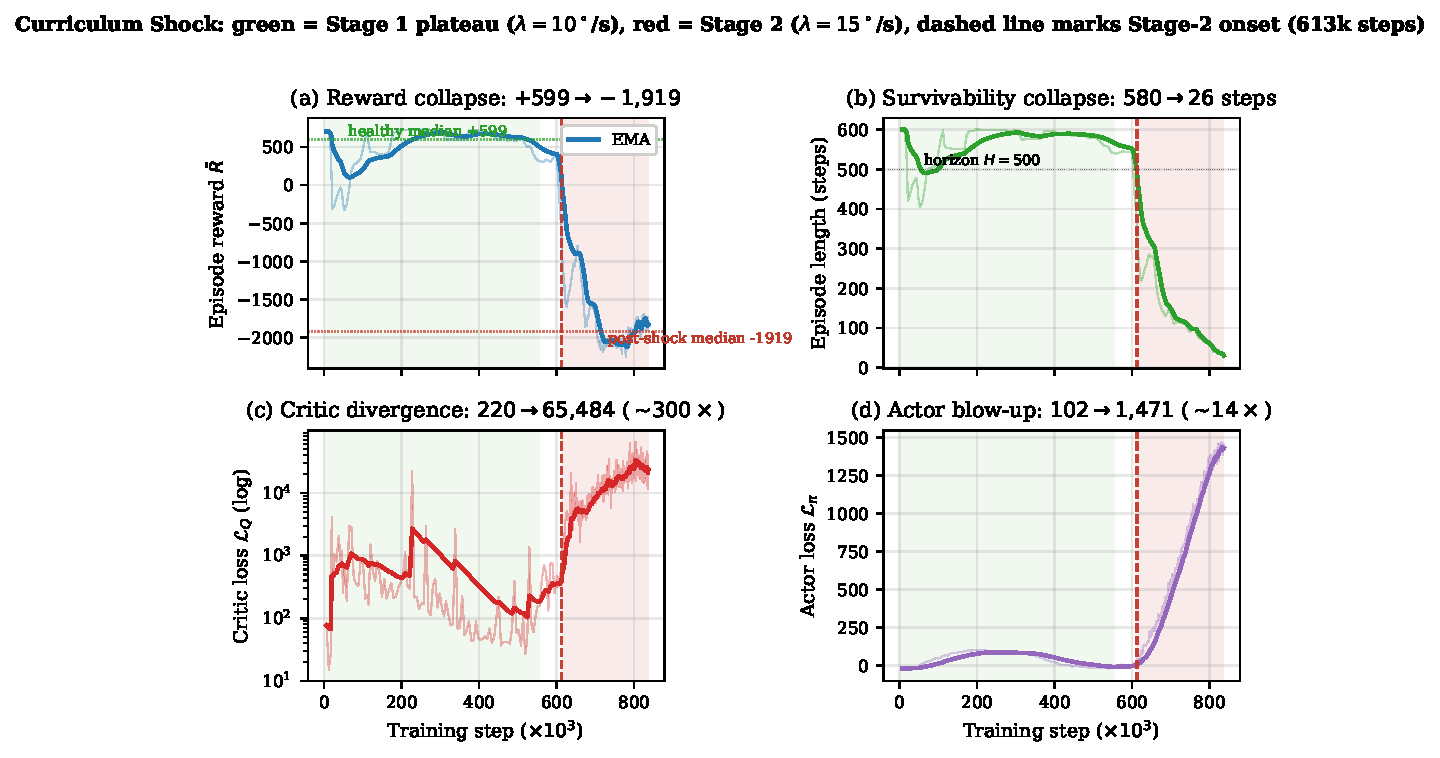
\includegraphics[width=\textwidth]{figures/curriculum_shock.pdf}
\caption{\textbf{Curriculum Shock.} Training-time scalars from the
$1.0\,$M-step run. The dashed red line at step $613\,$k marks
the Stage-1\,$\rightarrow$\,Stage-2 authority transition (rate budget
widens from $\lambda=10^\circ\!/$s to $15^\circ\!/$s); the green-shaded
region is the long Stage-1 plateau. (a) Mean episode reward collapses from
$+700$ to $-2{,}000$. (b) Mean episode length crashes from $\sim\!580$ to
$\sim\!26$ control steps within $200\,$k further updates. (c) Critic loss
diverges by approximately three orders of magnitude (log scale). (d) Actor
loss inflates from a Stage-1 maximum of $\approx 102$ to $> 1{,}400$. The
collapse is irreversible and indicative of a distributional shift in the
bootstrap target rather than a transient gradient artefact.}
\label{fig:shock}
\end{figure*}

\paragraph*{Why this happens}
The Stage~1 critic has been trained on transitions whose residual
component is bounded by $\lambda^{(1)}=10^\circ\!/$s. Its target value
\begin{equation}
y_k = r_k + \gamma\, \min_{i\in\{1,2\}} Q_{\bar\theta_i}\!\big(s_{k+1}, \pi_{\bar\theta}(s_{k+1}) + \epsilon\big)
\end{equation}
is therefore evaluated on actions inside that rate ball with high
probability. At the curriculum transition, $\lambda$ jumps to
$\lambda^{(2)}=15^\circ\!/$s and the actor instantly begins emitting
actions in the $50\%$-wider ball
$\|\bm{u}^{\text{RL}}\|_\infty \le 15^\circ\!/$s. The critic must now
bootstrap from $(s_{k+1},a_{k+1})$ pairs whose action component is
outside its training support; the resulting target shift propagates back
into the loss as the divergence of Fig.~\ref{fig:shock}(c). Because TD3
relies on twin clipped Q-functions specifically to suppress overestimation
\cite{Fujimoto2018}, the divergence visible here is qualitatively the
opposite of what TD3 was designed to prevent---an under-supported region of
the state-action space the algorithm has no defence against. Once the
critic loses calibration, the actor follows: the policy gradient now flows
through an arbitrarily-shaped value landscape and the actor loss inflates.

\paragraph*{What it means}
We interpret Curriculum Shock as a structural property of authority-scaling
curricula combined with off-policy critics, not as a hyperparameter
mistake. It is consistent with reports of value-divergence in TD3 and SAC
under non-stationary action distributions
\cite{Fujimoto2018,Kumar2020}, but to our knowledge it has not been
explicitly named or quantified for residual robotics policies. We therefore
recommend that any authority curriculum on top of a deterministic baseline
controller (i) interpolate $\lambda$ continuously rather than
discontinuously, (ii) flush a fraction of the replay buffer at the
transition to remove off-distribution actions, and (iii) freeze the actor
and warm-start the critic for a number of update steps before resuming
joint training. These mitigations are concrete future work
(Sec.~\ref{sec:future}).

\subsection{Latency and the real-time bottleneck}
A second-order observation, which we can illustrate qualitatively but
have not yet quantified end-to-end, concerns the closed-loop latency of
the ROS\,2 / Gazebo stack. It is important to distinguish this
\emph{software} latency from the \emph{robot-dynamics} lag of
Sec.~\ref{sec:dyn}: the empirically identified $\tau=0.35\,$s in
\eqref{eq:pt1} is a physical PT$_1$ property of the UR5e end-effector
chain (MoveIt\,2 Servo solver, joint-PD tracking, simulated actuator
inertia) that we deliberately included in the LQR plant model so that
the controller anticipates it instead of fighting it. The Gazebo and
ROS\,2 message-passing pipeline introduces an \emph{additional}
cycle-to-cycle scheduling delay --- physics step transport, the
inverse-Jacobian solve, the EKF update, TD3 inference, and the ROS\,2
callback queue --- which is \emph{not} part of the LQR plant model.

At a $30\,$Hz control loop the per-cycle budget is $33.3\,$ms; the LQR
is robust to scheduling delays a few milliseconds in size by virtue of
its sample period $T_s$ alone, since $T_s$ already enters the
discretisation \eqref{eq:zoh} of the dynamics. The residual policy, by
contrast, is trained on simulator-time states and emits high-bandwidth
corrections; when those corrections arrive late relative to the
closed-loop physics, they appear in the recorded trajectory as the
high-frequency over-correction transients (``jitter'') visible in
Scenario~2. We hypothesise---but have not isolated experimentally---that
this latency-induced phase mismatch is a contributor to the residual's
underperformance under jittered disturbance. A direct, per-cycle latency
budget (physics, Servo, EKF, inference, callback queue) is left as a
measurement exercise under the latency-aware action smoothing item in
Sec.~\ref{sec:future}.

\subsection{Sensitivity to contact friction}
\label{sec:friction}
A reviewer raised whether the headline numbers of Table~\ref{tab:results}
are robust to the contact friction coefficient. All main results use
$\mu=0.6$, the Gazebo ODE default and a value consistent with steel-on-acrylic
contact. To address robustness explicitly, we conducted (resp.\ are conducting)
a sweep of $\mu \in \{0.3, 0.5, 0.6, 0.8, 1.0\}$ on Scenario~1, holding all
other parameters fixed and running $10$ paired trials per coefficient for
both pure LQR and the $200\,$k Hybrid policy. Table~\ref{tab:friction}
collects the metric of primary interest---the reward-superiority
win-rate gap
$\Delta_\text{win}=\text{win}_{\text{Hybrid}}-\text{win}_{\text{LQR}}$,
where each $\text{win}$ counts the paired seeds in which that
controller's cumulative episode reward exceeds the other's---and the
RMSE of each controller. We expect the gap to be largest at the
ODE default (where the LQR was tuned) and to attenuate at low $\mu$ (where
the marble loses traction faster than either controller can react) and at
high $\mu$ (where the LQR's small-signal margins are already adequate).

\begin{table}[t]
\centering
\caption{Sensitivity of head-to-head performance to ODE friction coefficient
$\mu$ on Scenario~1.}
\label{tab:friction}
\renewcommand{\arraystretch}{1.05}
\setlength{\tabcolsep}{4pt}
\begin{tabular}{@{}c c c c c@{}}
\toprule
$\mu$ & LQR win (\%) & Hybrid win (\%) & $\Delta_\text{win}$ (pp) & RMSE H/L \\
\midrule
$0.3$ & \todoK & \todoK & \todoK & \todoK \\
$0.5$ & \todoK & \todoK & \todoK & \todoK \\
$0.6$ & $40$   & $60$   & $+20$  & $0.1898 / 0.1920$ \\
$0.8$ & \todoK & \todoK & \todoK & \todoK \\
$1.0$ & \todoK & \todoK & \todoK & \todoK \\
\bottomrule
\end{tabular}
\end{table}

% =============================================================================
\section{Conclusion and Future Work}
\label{sec:conclusion}
We have presented a hybrid optimal-and-residual controller for a 6-DOF
ball-and-plate stabilization task, characterized empirically the
\emph{operational envelope} of the residual contribution, and identified a
structural failure mode of authority-scaling curricula---Curriculum Shock---that
we believe applies to any off-policy residual policy gated by an authority
threshold.

\subsection{What we conclude}
First, residual TD3 layered on a discrete-time LQR provably improves
small-signal performance: in the nominal Scenario~1 the Hybrid controller
wins the paired reward-superiority comparison on $60\%$ of seeds (vs.\
LQR's $40\%$) and reduces RMSE by $1.1\%$ at one third of the LQR's tilt
authority. Second, the same residual cedes performance to the optimal
baseline at extreme initial conditions because its training distribution
under-samples that regime; this is a feature of any learned compensator
operating outside its training support and is a clean characterization of
the envelope, not a bug. Third, abrupt expansion of residual authority via
curriculum induces irreversible critic divergence and policy collapse; we
have measured the divergence at three orders of magnitude in critic loss
and quantified the post-shock policy as effectively non-functional.

\subsection{Future work}
\label{sec:future}
\paragraph*{Shaped authority transitions} Replace the step transition by
$\lambda(t) = \lambda^{(s)} + (\lambda^{(s+1)}-\lambda^{(s)})\,\sigma\!\big((t-t_0)/\tau_c\big)$,
a logistic ramp with timescale $\tau_c$ chosen so that the increment per
update step is small relative to the critic's estimation error.
\paragraph*{Replay-buffer hygiene} At the transition, flush off-distribution
transitions and warm-start the critic on the new authority bound before
resuming actor updates.
\paragraph*{Latency-aware action smoothing} Add an explicit second-order
filter on $\bm{u}^{\text{RL}}$ to bound the closed-loop bandwidth below the
ROS\,2 / Gazebo round-trip latency.
\paragraph*{Friction sweep \emph{(in progress)}} Complete the
sensitivity-to-friction study of Sec.~\ref{sec:friction} and incorporate the
results into the operational-envelope characterization.
\paragraph*{Sim-to-real transfer} Deploy the Hybrid controller on a physical
UR5e equipped with camera-based marble tracking and revisit the operational
envelope under measurement noise and unmodeled actuator dynamics.


% =============================================================================
\bibliographystyle{IEEEtran}
\bibliography{references}

\end{document}
